\chapter{Discussion}
Please tell more about conclusion and how to the next work of this study.
\section{Mhd Zulfikar Akram Nastuion / 1164081}
\subsection{Teori}
\begin{enumerate}

\item Jelaskan kenapa file teks harus di lakukan tokenizer. Dilengkapi dengan ilustrasi atau gambar !
\par
Sebelumnya kita harus tau terlebih dahulu apa itu Tokenizer. Tokenizer adalah sebuah proses pembagian terhadap kalimat yang berada dalam dokumen sehingga menjadi sebuah bagian - bagian kata atau bisa kita sebut denga token. Dalam dataset Youtube Tokenizer digunakan untuk melakukan vektorisasi data, sehingga dapat kita simpulkan bahwa data yang telah kita buat dokumen pada chapter 6 yaitu data spam dan bukan spam akan dilakukan vektorisasi dengan menggunakan Tokenizer ini. Ilustrasi sederhana mengenai Tokenizer ini misalkan saya memiliki sebuah kalimat Nama Saya Adalah Yusniar jika gunakan fungsi Tokenizer ini akan dipecah menjadi kata per kata, perhatikan figure \ref{1}.

	\begin{figure}[!htbp!]
		\centerline{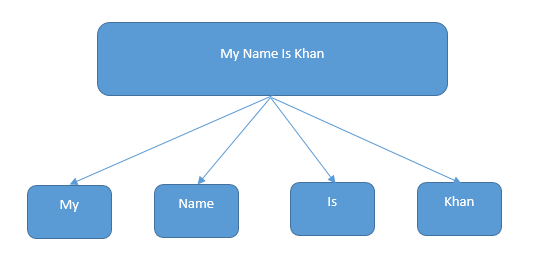
\includegraphics[width=0.5\textwidth]{figures/zulfikar/7/Teori/1164081_1.png}}
		\caption{Contoh Tokenizer.}
		\label{1}
	\end{figure}
\end{enumerate}